%% abtex2-modelo-trabalho-academico.tex, v-1.9.6 laurocesar
%% Copyright 2012-2016 by abnTeX2 group at http://www.abntex.net.br/ 
%%
%% This work may be distributed and/or modified under the
%% conditions of the LaTeX Project Public License, either version 1.3
%% of this license or (at your option) any later version.
%% The latest version of this license is in
%%   http://www.latex-project.org/lppl.txt
%% and version 1.3 or later is part of all distributions of LaTeX
%% version 2005/12/01 or later.
%%
%% This work has the L PPL maintenance status `maintained'.
%% 
%% The Current Maintainer of this work is the abnTeX2 team, led
%% by Lauro César Araujo. Further information are available on 
%% http://www.abntex.net.br/
%%
%% This work consists of the files abntex2-modelo-trabalho-academico.tex,
%% abntex2-modelo-include-comandos and abntex2-modelo-references.bib

% ------------------------------------------------------------------------
% ------------------------------------------------------------------------
% abnTeX2: Modelo de Trabalho Academico (tese de doutorado, dissertacao de
% mestrado e trabalhos monograficos em geral) em conformidade com 
% ABNT NBR 14724:2011: Informacao e documentacao - Trabalhos academicos -
% Apresentacao
% ------------------------------------------------------------------------
% ------------------------------------------------------------------------

\documentclass[
	12pt,				% tamanho da fonte
	openright,			% capítulos começam em pág ímpar (insere página vazia caso preciso)
	twoside,			% para impressão em recto e verso. Oposto a oneside
	a4paper,			% tamanho do papel. 
	chapter=TITLE,		% títulos de capítulos convertidos em letras maiúsculas
	section=TITLE,		% títulos de seções convertidos em letras maiúsculas
	sumario=abnt-6027-2012,
	english,			% idioma adicional para hifenização
	brazil				% o último idioma é o principal do documento
	]{abntex2}

\usepackage{udescCCT} 	% Pacote de customizações da UDESC/CCT

% ----------------------------------------------------------
% Pacotes básicos 
% ----------------------------------------------------------
\usepackage{amsmath}							% Pacote matemático
\usepackage{amssymb}							% Pacote matemático
\usepackage{amsfonts}							% Pacote matemático
\usepackage{lmodern}							% Usa a fonte Latin Modern			
\usepackage[T1]{fontenc}						% Selecao de codigos de fonte.
\usepackage[utf8]{inputenc}						% Codificacao do documento (conversão automática dos acentos)
\usepackage{lastpage}							% Usado pela Ficha catalográfica
\usepackage{indentfirst}						% Indenta o primeiro parágrafo de cada seção.
\usepackage[dvipsnames,table]{xcolor}			% Controle das cores
\usepackage{graphicx}							% Inclusão de gráficos
\usepackage{microtype} 							% para melhorias de justificação
\usepackage{lipsum}								% para geração de dummy text
\usepackage[brazilian,hyperpageref]{backref}	% Paginas com as citações na bibl
\usepackage[alf]{abntex2cite}					% Citações padrão ABNT
%\usepackage[num]{abntex2cite}					% Citações padrão ABNT numérica
\usepackage{adjustbox}							% Pacote de ajuste de boxes
\usepackage{subcaption}							% Inclusão de Subfiguras e sublegendas		
\usepackage{enumitem}							% Personalização de listas
\usepackage{siunitx}							% Grandezas e unidades
\usepackage[section]{placeins}					% Manter as figuras delimitadas na respectiva seção com a opção [section]
\usepackage{multirow}							% Multi colunas nas tabelas
\usepackage{array,tabularx} 					% Pacotes de tabelas
\usepackage{booktabs}							% Pacote de tabela profissonal
\usepackage{rotating}							% Rotacionar figuras e tabelas
\usepackage{xfrac}								% Fazer frações n/d em linha
\usepackage{bm}									% Negrito em modo matemático
\usepackage{xstring}							% Manipulação de strings
\usepackage{pgfplots}							% Pacote de Gráficos
\usepackage{tikz}								% Pacote de Figuras
\usepackage[american, cuteinductors,smartlabels, fulldiode, siunitx, americanvoltages, oldvoltagedirection, smartlabels]{circuitikz}						% Pacote de circuitos elétricos

% Personalização das opções das listas
\setlist[itemize]{leftmargin=\parindent}

% Citação online --- MODIFICAR ---
\newcommand{\citeshort}[1]{\citeauthoronline{#1}~(\citeyear{#1})}

\newcommand{\me}[1]{Elaborado pelo autor, #1.}

% Configuração do pgfplots
\pgfplotsset{compat=newest} %compat=1.14
\pgfplotsset{plot coordinates/math parser=false} 
\newlength\figureheight 
\newlength\figurewidth 

% Libraries do TiKz
\usetikzlibrary{quotes,angles,arrows}
\usetikzlibrary{through,calc,math}
\usetikzlibrary{graphs,backgrounds,fit}
\usetikzlibrary{shapes,positioning,patterns,shadows}
\usetikzlibrary{decorations.pathreplacing}
\usetikzlibrary{shapes.geometric}
\usetikzlibrary{arrows.meta}
\usetikzlibrary{external}

%\tikzexternalize[]
%\tikzexternalenable
%\tikzexternalize
%\tikzexternaldisable
%\tikzset{external/force remake}
%\tikzexternalize[shell escape=-enable-write18]

% Configurações do CircuiTiKz
\ctikzset{bipoles/thickness=1}
%\ctikzset{bipoles/length=1.2cm}
\ctikzset{monopoles/ground/width/.initial=.2}
\ctikzset{bipoles/resistor/height=0.25}
\ctikzset{bipoles/resistor/width=0.6}
\ctikzset{bipoles/capacitor/height=0.5}
\ctikzset{bipoles/capacitor/width=0.15}
\ctikzset{bipoles/generic/height=0.25}
\ctikzset{bipoles/generic/width=0.6}
%\ctikzset{bipoles/capacitor polar/length=0.5}
%\ctikzset{bipoles/diode/height=.375}
%\ctikzset{bipoles/diode/width=.3}
%\ctikzset{tripoles/thyristor/height=.8}
%\ctikzset{tripoles/thyristor/width=1}
\ctikzset{bipoles/vsourcesin/height=.5}
\ctikzset{bipoles/vsourcesin/width=.5}
\ctikzset{bipoles/cvsourceam/height=.6}
\ctikzset{bipoles/cvsourceam/width=.6}
%\ctikzset{tripoles/european controlled voltage source/width=.4}

\tikzstyle{every node}=[font=\footnotesize]
\tikzstyle{every path}=[line width=0.25pt,line cap=round,line join=round]
%\tikzstyle{every path}=[line cap=round,line join=round]


% Definição de cores MATLAB
\definecolor{matlab_blue}{rgb}	{         0,    0.4470,    0.7410}
\definecolor{matlab_orange}{rgb}{    0.8500,    0.3250,    0.0980}
\definecolor{matlab_yellow}{rgb}{    0.9290,    0.6940,    0.1250}
\definecolor{matlab_violet}{rgb}{    0.4940,    0.1840,    0.5560}
\definecolor{matlab_green}{rgb}	{	 0.4660,    0.6740,    0.1880}
\definecolor{matlab_lblue}{rgb}	{    0.3010,    0.7450,    0.9330}
\definecolor{matlab_red}{rgb}	{    0.6350,    0.0780,    0.1840}

% Personalização das legendas
\usepackage[format = hang,
			labelsep = endash,
			singlelinecheck = false,
			skip = 6pt,
			listformat = simple]{caption}	

% Personalização das unidades
\sisetup{output-decimal-marker = {,}}
\sisetup{exponent-product = \cdot, output-product = \cdot}
\sisetup{tight-spacing=true}
\sisetup{group-digits = false}

% Personalizações de tipo de colunas de tabelas
\newcolumntype{L}[1]{>{\raggedright\let\newline\\\arraybackslash\hspace{0pt}}m{#1}}
\newcolumntype{C}[1]{>{\centering\let\newline\\\arraybackslash\hspace{0pt}}m{#1}}
\newcolumntype{R}[1]{>{\raggedleft\let\newline\\\arraybackslash\hspace{0pt}}m{#1}}

% Personalizações de cores da UDESC
\definecolor{CapaAmareloUDESC}{RGB}{243,186,83}		% Especializacao
\definecolor{CapaVerdeUDESC}{RGB}{0,112,52}			% Mestrado
\definecolor{CapaVermelhoUDESC}{RGB}{171,35,21}		% Doutorado
\definecolor{CapaAzulUDESC}{RGB}{38,54,118} 		% Pós-Doutorado

% CONFIGURAÇÕES DE PACOTES
% Configurações do pacote backref
% Usado sem a opção hyperpageref de backref
\renewcommand{\backrefpagesname}{Citado na(s) página(s):~}
% Texto padrão antes do número das páginas
\renewcommand{\backref}{}
% Define os textos da citação
\renewcommand*{\backrefalt}[4]{
	\ifcase #1 %
	Nenhuma citação no texto.%
	\or
	Citado na página #2.%
	\else
	Citado #1 vezes nas páginas #2.%
	\fi}%

% alterando o aspecto da cor azul
%\definecolor{blue}{RGB}{41,5,195}

% informações do PDF
\makeatletter
\hypersetup{
	%pagebackref=true,
	pdftitle={\@title}, 
	pdfauthor={\@author},
	pdfsubject={\imprimirpreambulo},
	pdfcreator={LaTeX with abnTeX2},
	pdfkeywords={abnt}{latex}{abntex}{abntex2}{trabalho academico}, 
	colorlinks=true,       		% false: boxed links; true: colored links
	linkcolor=black,          	% color of internal links
	citecolor=black,        	% color of links to bibliography
	filecolor=black,      		% color of file links
	urlcolor=black,
	bookmarksdepth=4
}
\makeatother


\makeatletter
\newcommand{\includetikz}[1]{%
	\tikzsetnextfilename{#1}%
	\input{#1.tex}%
}
\makeatother

% Espaçamento depois do título
\setlength{\afterchapskip}{0.7\baselineskip}
% O tamanho do parágrafo é dado por:
\setlength{\parindent}{1.25cm}
% Controle do espaçamento entre um parágrafo e outro:
\setlength{\parskip}{0.15cm}  % tente também \onelineskip
%\SingleSpacing % Espaçamento simples 
\OnehalfSpacing % Espaçamento 1,5 (UDESC/CCT)
%\DoubleSpacing	% Espaçamento duplo

% ---
% Margens - NBR 14724/2011 - 5.1 Formato
% ---
\setlrmarginsandblock{3cm}{2cm}{*}
\setulmarginsandblock{3cm}{2cm}{*}
\checkandfixthelayout[fixed]
% ---


% To use externalize consider
%https://tex.stackexchange.com/questions/182783/tikzexternalize-not-compatible-with-miktex-2-9-abntex2-package
%Lauro Cesar digged into the problem until he came with a solution for me to test. And it Works!
%
%According to this link:
%
%The package calc changed the commands \setcounter and friends to be fragile. So you have to make them robust. The example below uses etoolbox with \robustify:
%
\usepackage{etoolbox}
\robustify\setcounter
\robustify\addtocounter
\robustify\setlength
\robustify\addtolength


%% How to silence memoir class warning against the use of caption package?
%% https://tex.stackexchange.com/questions/391993/how-to-silence-memoir-class-warning-against-the-use-of-caption-package
%\usepackage{silence}
%\WarningFilter*{memoir}{You are using the caption package with the memoir class}
%\WarningFilter*{Class memoir Warning}{You are using the caption package with the memoir class}





	% Incliu pacotes básicos 

% -----------------------------------------------------------------
% Você pode adicionar seus pacotes a partir desta linha;
% -----------------------------------------------------------------

%\usepackage[showframe,pass]{geometry}
%\usepackage[11,12]{pagesel}


% -----------------------------------------------------------------
% Informações de dados para CAPA e FOLHA DE ROSTO
% -----------------------------------------------------------------

\titulo{teste2343}%

\autor{Nome do Autor {}Sobrenome}%
\orientador{Nome do orientador {}do Sobrenome}%
\coorientador{Nome do coorientador {}Sobrenome}%

% ATENÇÃO: O símbolo {} indica o sobrenome para a ficha catalográfica.
% Exemplo: Sherlock Holmes {}da Silva para sobrenomes compostos;
% Exemplo: Arnold Alois {}Schwarzenegger para sobrenome simples.

\instituicao{Universidade do Estado de Santa Catarina, Centro de Ciências Tecnológicas, Programa de Pós--Graduação em Engenharia Elétrica}%

%\tipotrabalho{Tese (Doutorado)}
\tipotrabalho{Dissertação (Mestrado)}

%\preambulo{Tese apresentada ao Programa de Pós--Graduação em Engenharia Elétrica do Centro de Ciências Tecnológicas da Universidade do Estado de Santa Catarina, como requisito parcial para a obtenção do grau de Doutor em Engenharia Elétrica.}

\preambulo{Dissertação apresentada ao Programa de Pós--Graduação em Engenharia Elétrica do Centro de Ciências Tecnológicas da Universidade do Estado de Santa Catarina, como requisito parcial para a obtenção do grau de Mestre em Engenharia Elétrica.}

\local{Joinville}%
\data{\the\year}%
% ---

% compila o indice
\makeindex

% -----------------------------------------------------------------
% Início do documento
% -----------------------------------------------------------------
\begin{document}

\selectlanguage{brazil}
\frenchspacing  % Retira espaço extra obsoleto entre as frases.

% -----------------------------------------------------------------
% ELEMENTOS PRÉ-TEXTUAIS
% -----------------------------------------------------------------
\pretextual

% Você pode comentar os elementos que não deseja em seu trabalho;

% A capa pode ser escolhida dentro do arquivo Capa.tex (TCC, Master, Doc, ...)
% ---
% Capa
% ---

%\imprimircapa				% Capa padrão
%\imprimircapaTCC			% Capa UDESC para TCC
\imprimircapaDissertacao	% Capa UDESC para Dissertações
%\imprimircapaTese			% Capa UDESC para Teses
%\imprimircapaPosDoc		% Capa UDESC para Pós-Doutorado

					% Elemento Obrigatório
% ---
% Folha de rosto
% (o * indica que haverá a ficha bibliográfica)
% ---
\imprimirfolhaderosto
% ---

			% Elemento Obrigatório
% Caso não utilize a Ficha Catalográfica entre na folha de rosto e retire o *

% ---
% Inserir a ficha bibliografica
% ---

% Isto é um exemplo de Ficha Catalográfica, ou ``Dados internacionais de
% catalogação-na-publicação''. Você pode utilizar este modelo como referência. 
% Porém, provavelmente a biblioteca da sua universidade lhe fornecerá um PDF
% com a ficha catalográfica definitiva após a defesa do trabalho. Quando estiver
% com o documento, salve-o como PDF no diretório do seu projeto e substitua todo
% o conteúdo de implementação deste arquivo pelo comando abaixo:



% \begin{fichacatalografica}
%     \includepdf{fig_ficha_catalografica.pdf}
% \end{fichacatalografica}


%	\setlength{\parindent}{0cm}
%	\setlength{\parskip}{0pt}
\begin{fichacatalografica}
	%\sffamily
	%\rmfamily
	\ttfamily \hbadness=10000
	\vspace*{\fill}					% Posição vertical
	\begin{center}					% Minipage Centralizado
%	\begin{minipage}[c]{8cm}
%	\centering \sffamily
%	 Ficha catalográfica elaborada pelo(a) autor(a), com auxílio do programa de geração automática da Biblioteca Setorial do CCT/UDESC
%	\end{minipage}
	\fbox{\begin{minipage}[c]{12.5cm}		% Largura
	\flushright
	{\begin{minipage}[c]{10.5cm}		% Largura
	\vspace{1.25cm}
	%\footnotesize
	\setlength{\parindent}{1.5em}
	\noindent \invertname{\imprimirautor} \par
	\imprimirtitulo{ }/{ }\imprimirautor. -- \imprimirlocal, \imprimirdata .\par
	\pageref{LastPage} p. : il. ; 30 cm.\par
	\vspace{1.5em}
	\imprimirorientadorRotulo~\imprimirorientador\par
	\imprimircoorientadorRotulo~\imprimircoorientador\par
	\imprimirtipotrabalho~--~\imprimirinstituicao, \imprimirlocal, \imprimirdata.\par
	\vspace{1.5em}
		1. Palavra-chave.
		2. Palavra-chave.
		3. Palavra-chave.
 		4. Palavra-chave.
		5. Palavra-chave.
		I. \invertname{\imprimirorientador}. 
		II. \invertname{\imprimircoorientador}.
		III. \imprimirinstituicao .
		IV. Título %
	\vspace{1.25cm}	%		
	\end{minipage}%
	}% 
	\end{minipage}}%
	\end{center}
\end{fichacatalografica}


%\begin{fichacatalografica}
%	\sffamily
%	\vspace*{\fill}					% Posição vertical
%	\begin{center}					% Minipage Centralizado
%	\fbox{\begin{minipage}[c][8cm]{13.5cm}		% Largura
%	\small
%	\imprimirautor
%	%Sobrenome, Nome do autor
%	
%	\hspace{0.5cm} \imprimirtitulo  / \imprimirautor. --
%	\imprimirlocal, \imprimirdata-
%	
%	\hspace{0.5cm} \pageref{LastPage} p. : il. (algumas color.) ; 30 cm.\\
%	
%	\hspace{0.5cm} \imprimirorientadorRotulo~\imprimirorientador\\
%	
%	\hspace{0.5cm}
%	\parbox[t]{\textwidth}{\imprimirtipotrabalho~--~\imprimirinstituicao,
%	\imprimirdata.}\\
%	
%	\hspace{0.5cm}
%		1. Palavra-chave1.
%		2. Palavra-chave2.
%		3. Palavra-chave3.
% 		4. Palavra-chave4.
%		5. Palavra-chave5.
%		I. Orientador.
%		II. Universidade xxx.
%		III. Faculdade de xxx.
%		IV. Título 			
%	\end{minipage}}
%	\end{center}
%\end{fichacatalografica}
% ---

	% Elemento Obrigatório (Verso da Folha)
%
% ---
% Inserir errata
% ---
\begin{errata}
Elemento opcional da \citeonline[4.2.1.2]{NBR14724:2011}. Exemplo:

\vspace{\onelineskip}

FERRIGNO, C. R. A. \textbf{Tratamento de neoplasias ósseas apendiculares com
reimplantação de enxerto ósseo autólogo autoclavado associado ao plasma
rico em plaquetas}: estudo crítico na cirurgia de preservação de membro em
cães. 2011. 128 f. Tese (Livre-Docência) - Faculdade de Medicina Veterinária e
Zootecnia, Universidade de São Paulo, São Paulo, 2011.

\begin{table}[htb]
\center
\footnotesize
\begin{tabular}{|p{1.4cm}|p{1cm}|p{3cm}|p{3cm}|}
  \hline
   \textbf{Folha} & \textbf{Linha}  & \textbf{Onde se lê}  & \textbf{Leia-se}  \\
    \hline
    1 & 10 & auto-conclavo & autoconclavo\\
   \hline
\end{tabular}
\end{table}

\end{errata}
% ---				% Elemento Opcional
% ---
% Inserir folha de aprovação
% ---

% Isto é um exemplo de Folha de aprovação, elemento obrigatório da NBR
% 14724/2011 (seção 4.2.1.3). Você pode utilizar este modelo até a aprovação
% do trabalho. Após isso, substitua todo o conteúdo deste arquivo por uma
% imagem da página assinada pela banca com o comando abaixo:
%
% \includepdf{folhadeaprovacao_final.pdf}
%
\begin{folhadeaprovacao}



\begin{center}
	{\MakeTextUppercase{\ABNTEXchapterfont\large\imprimirautor}}

    \vspace*{\fill} %\vspace*{\fill}
    \begin{center}
      {\MakeTextUppercase{\ABNTEXchapterfont\bfseries\large\imprimirtitulo}}
    \end{center}
    \vspace*{\fill}
    
    %\hspace{.45\textwidth}
    {\begin{minipage}[c]{1\linewidth}
	    \setlength{\parindent}{1.25cm}
    	\imprimirpreambulo
    \end{minipage}}%
    \vspace*{\fill}
    \end{center}
        
	 
    {\bfseries Banca Examinadora: }
    \vspace*{\fill}
    
	{Orientador: \vspace{-16pt} }
    \assinatura{\textbf{Prof. \imprimirorientador , Dr.} \\ Univ. XXX} 
    {Coorientador: \vspace{-16pt}}   
    \assinatura{\textbf{Prof. \imprimircoorientador , Dr.} \\ Univ. XXX}
   
    {Membros: \vspace{-16pt} } 
    
% --- Exemplo de assinaturas em sequência ---       
	\setlength{\ABNTEXsignwidth}{8.5cm}
	
    \assinatura{\textbf{Prof. Professor, Dr.} \\ Univ. XXX}
    \assinatura{\textbf{Prof. Professor, Dr.} \\ Univ. XXX}
    \assinatura{\textbf{Prof. Professor, Dr.} \\ Univ. XXX}

% --- Exemplo de assinaturas lado a lado ---
	\setlength{\ABNTEXsignwidth}{7.5cm}
%
%    \noindent\hfill\assinatura*{\textbf{Prof. Professor, Dr.} \\ Univ. XXX}%
%    \hfill%
%    \assinatura*{\textbf{Prof. Professor, Dr.} \\ Univ. XXX}%
%    \hfill
%    
%    \noindent\hfill\assinatura*{\textbf{Prof. Professor, Dr.} \\ Univ. XXX}%
%    \hfill%
%    \assinatura*{\textbf{Prof. Professor, Dr.} \\ Univ. XXX}%
%    \hfill
    
    \vspace*{\fill}  
    \begin{center}
    {\large\imprimirlocal, 01 de maio de \imprimirdata}
	\end{center}
    \vspace*{1cm}  
\end{folhadeaprovacao}
% ---		% Elemento Obrigatório
% ---
% Dedicatória
% ---
\begin{dedicatoria}
   \vspace*{\fill}
   \centering
   \noindent
   \textit{ Este trabalho é dedicado às crianças adultas que,\\
   quando pequenas, sonharam em se tornar cientistas.} \vspace*{\fill}
\end{dedicatoria}
% ---
			% Elemento Opcional
% ---
% Agradecimentos
% ---
\begin{agradecimentos}
Os agradecimentos principais são direcionados à Gerald Weber, Miguel Frasson,
Leslie H. Watter, Bruno Parente Lima, Flávio de Vasconcellos Corrêa, Otavio Real
Salvador, Renato Machnievscz\footnote{Os nomes dos integrantes do primeiro
projeto abn\TeX\ foram extraídos de
\url{http://codigolivre.org.br/projects/abntex/}} e todos aqueles que
contribuíram para que a produção de trabalhos acadêmicos conforme
as normas ABNT com \LaTeX\ fosse possível.

Agradecimentos especiais são direcionados ao Centro de Pesquisa em Arquitetura
da Informação\footnote{\url{http://www.cpai.unb.br/}} da Universidade de
Brasília (CPAI), ao grupo de usuários
\emph{latex-br}\footnote{\url{http://groups.google.com/group/latex-br}} e aos
novos voluntários do grupo
\emph{\abnTeX}\footnote{\url{http://groups.google.com/group/abntex2} e
\url{http://www.abntex.net.br/}}~que contribuíram e que ainda
contribuirão para a evolução do \abnTeX.

\end{agradecimentos}
% ---		% Elemento Opcional
% ---
% Epígrafe
% ---
\begin{epigrafe}
    \vspace*{\fill}
	\begin{flushright}
		\textit{``Não vos amoldeis às estruturas deste mundo, \\
		mas transformai-vos pela renovação da mente, \\
		a fim de distinguir qual é a vontade de Deus: \\
		o que é bom, o que Lhe é agradável, o que é perfeito.\\
		(Bíblia Sagrada, Romanos 12, 2)}
	\end{flushright}
\end{epigrafe}
% ---				% Elemento Opcional
% ---
% RESUMOS
% ---

% resumo em português
\setlength{\absparsep}{18pt} % ajusta o espaçamento dos parágrafos do resumo
\begin{resumo}
 Segundo a \citeonline[3.1-3.2]{NBR6028:2003}, o resumo deve ressaltar o
 objetivo, o método, os resultados e as conclusões do documento. A ordem e a extensão
 destes itens dependem do tipo de resumo (informativo ou indicativo) e do
 tratamento que cada item recebe no documento original. O resumo deve ser
 precedido da referência do documento, com exceção do resumo inserido no
 próprio documento. (\ldots) As palavras-chave devem figurar logo abaixo do
 resumo, antecedidas da expressão Palavras-chave:, separadas entre si por
 ponto e finalizadas também por ponto.

 \textbf{Palavras-chave}: latex. abntex. editoração de texto.
\end{resumo}
				% Elemento Obrigatório
% ---
% Abstract
% ---

% resumo em inglês
\begin{resumo}[Abstract]
 \begin{otherlanguage*}{english}
   This is the english abstract.

   \vspace{\onelineskip}
 
   \noindent 
   \textbf{Keywords}: latex. abntex. text editoration.
 \end{otherlanguage*}
\end{resumo}
				% Elemento Obrigatório

% ---
% inserir lista de ilustrações
% ---
\pdfbookmark[0]{\listfigurename}{lof}
\listoffigures*
\cleardoublepage
% ---

% ---
% inserir lista de tabelas
% ---
%\pdfbookmark[0]{\listtablename}{lot}
%\listoftables*
%\cleardoublepage
% ---

% ---
% inserir lista de abreviaturas e siglas
% ---
%\begin{siglas}
%  \item[ABNT] Associação Brasileira de Normas Técnicas
%  \item[abnTeX] ABsurdas Normas para TeX
%\end{siglas}
% ---

% ---
% inserir lista de símbolos
% ---
%\begin{simbolos}
%  \item[$ \Gamma $] Letra grega Gama
%  \item[$ \Lambda $] Lambda
%  \item[$ \zeta $] Letra grega minúscula zeta
%  \item[$ \in $] Pertence
%\end{simbolos}
% ---
				% Elemento Opcional
% ---
% inserir o sumario
% ---
\pdfbookmark[0]{\contentsname}{toc}
\tableofcontents*
\cleardoublepage
% ---
				% Elemento Obrigatório



% -----------------------------------------------------------------
% ELEMENTOS TEXTUAIS
% -----------------------------------------------------------------
\textual

% Mantenha está estrutura, assim você deixa o trabalho mais organizado


%\chapter{Introdução}


\chapter{Apresentação Gráfica}

É apresentado um resumo das normas para trabalhos acadêmicos da UDESC.

\section{Margens}

As margens devem seguir os seguintes padrões:

\begin{itemize}
\item Superior: 3,0 cm
\item Inferior: 2,0 cm
\item Interna: 3,0 cm
\item Externa: 2,0 cm
\end{itemize}

Parágrafo: a 1,25 cm da margem esquerda.

\section{Formatação do Papel e Fonte}

Papel branco, formato A4 (\SI{21}{cm} $\times$ \SI{29,7}{cm}), gramatura 75 com texto em cor preta 

\textbf{Elementos pré-textuais}: iniciar no anverso da página, com exceção da ficha catalográfica que deve vir no verso da folha de rosto.

Os elementos textuais e pós-textuais devem ser digitados no anverso e verso das páginas, com exceção das páginas que derem início as seções primárias, que devem ser no anverso das páginas.


\textbf{Formato}: Arial ou Times New Roman.

\textbf{Tamanho 12}: elementos pré-textuais, textuais e pós-textuais

\textbf{Tamanho 10}: citações longas, notas de rodapé, legendas das ilustrações, tabelas e paginação.

Obs.: A fonte tamanho 12 pt deve ser usada em todo o trabalho, inclusive títulos das seções e
subseções.

\section{ESPAÇAMENTO E PARÁGRAFOS}

O texto do corpo do trabalho deve ser \textbf{alinhado à esquerda e à direita (justificado)}, digitado
em \textbf{espaço de 1,5 linha}, em \textbf{fonte tamanho 12 }(com exceção das referências e citações, tratados adiante), incluindo apêndices e anexos

Citações longas devem ter um recuo de 4,0 cm da margem esquerda, espaço simples e fonte
em tamanho 10.

Notas de rodapé, legendas e fontes de ilustrações e tabelas devem ser apresentadas em
espaço simples (1,0 linha), em fonte tamanho 10.

As referências no final do trabalho devem ser alinhadas somente à margem esquerda,
separadas uma das outras por espaço duplo; entre as linhas da mesma referência deve ser usado
espaço simples.

Os títulos principais (seção primária) devem ser separados do texto por 1 (um) espaço de 1,5
linha em branco. Títulos não numerados devem ser centralizados, títulos numerados devem ser
alinhados à esquerda. A numeração deve ser separada dos títulos ou subtítulos por um espaço de
caractere (sem ponto).

Os títulos principais devem ser alinhados pela margem superior da mancha, sendo
apresentados sempre em nova página. Os subtítulos (seções secundárias, terciárias, etc.) devem
aparecer na sequência do texto (sem iniciar nova página), separados do texto anterior e posterior
por 1 (um) espaço de 1,5 linha em branco.

\section{Paginação}

Todas as páginas do trabalho, a \textbf{partir da folha de rosto}, devem ser contadas sequencialmente,
mas nem todas são numeradas. A numeração é colocada a partir da \textbf{primeira página da parte textual (Introdução)}, em algarismos arábicos, fonte 10.

No verso da página (páginas pares) o número de página é inserido dentro da margem
esquerda superior. No anverso da página (páginas ímpares) o número é inserido na margem direita
superior. Dessa forma, o número da página estará sempre na margem externa da mancha gráfica.

\section{Figuras}

As ilustrações devem ser colocadas após sua citação no texto, deixando-se um espaço
(1,5) entre o texto e a figura. Após, o texto prossegue a um espaço (1,5).

\textbf{Identificação}: parte superior, precedida da palavra designativa, número de ordem de
ocorrência no texto, em algarismos arábicos, travessão e título. Espaçamento
entrelinhas simples e fonte 12. Se o título ocupar mais de uma linha, a segunda linha
deverá iniciar abaixo da primeira palavra do título.

\textbf{Fonte (identificador do responsável)}: na parte inferior da ilustração deve-se indicar a
fonte consultada (elemento obrigatório, mesmo que seja elaborado pelo autor).
Apresentar a fonte consultada precedida da palavra Fonte em letra maiúscula e
minúscula, dois pontos e a fonte, em tamanho 10 pt.

Todas as ilustrações deverão ser \textbf{centralizadas} em relação a margem.

Se o espaço da página não permitir, a ilustração deve aparecer na página seguinte,
enquanto o texto prossegue normalmente no restante da página anterior.

Na Fig.~\ref{fig:marca_udesc_01} pode ser observada uma figura de exemplo.

\begin{figure}[!htbp]
	\centering	
 	\caption{Marca UDESC.}
	
\includegraphics[width=0.5\textwidth]{cor_horizontal_pdf.pdf}
	\fonte{Elaborado pelo autor, \the\year.}	
	\label{fig:marca_udesc_01}
\end{figure}

\begin{figure}[!htbp]
\flushleft 
	\caption{Outras marcas da UDESC.}
	\begin{subfigure}[b]{0.5\linewidth}
		\centering
		
\includegraphics[width=0.5\textwidth]{cor_vertical_pdf.pdf}
		\caption{Tipo de marca 01}
	\end{subfigure}%
	\begin{subfigure}[b]{0.5\linewidth}
		\centering
		
\includegraphics[width=0.85\textwidth]{cor_horizontal_ass_1_pdf.pdf}
		\caption{Marca com descrição da UDESC.}
	\end{subfigure}
	\fonte{Retirado de (UDESC, 2018).}	
\end{figure}

\section{Tabelas}

A largura das tabelas e quadros, não poderá ultrapassar a configuração das margens esquerda
e direita do texto. Deve-se ajustar o tamanho das tabelas e quadros ao conteúdo.

Devem estar configurados em \textbf{espaçamento simples}, com \textbf{fonte 10 ou 12 pt}, e seguir o mesmo
padrão em todo o trabalho.

Com relação a formatação, a tabela apresenta os seguintes elementos: título, cabeçalho,
conteúdo, fonte e, se necessário, nota(s) explicativa(s) (geral e/ou específica).

As informações inseridas em uma tabela devem ser divididas por linhas na horizontal, porém as \textbf{bordas laterais não podem ser fechadas}.

Na Tabela~\ref{tab:tabela_exemplo} pode ser observada uma tabela de exemplo.

\begin{table}[!htbp]
\centering
\small
\renewcommand{\arraystretch}{1.1}
\caption{Parâmetros de comunicação entre o CCS e o ESP8266.}%
\label{tab:tabela_exemplo}
\begin{tabular}{C{4cm} | C{4cm} | C{4cm}}
\toprule
 & \multicolumn{2}{c}{\textbf{Dispositivos}} \\
\cmidrule(lr{0.5ex}){2-3}
\multirow{-2}{*}[2pt]{\textbf{Parâmetros}}	& \textbf{CCS}	& \textbf{ESP} \\ 
\midrule
Endereço IP 			& 192.168.137.01 	& 192.168.137.212  		\\
Porta de recebimento 	& 9001 				& 9001  				\\
Porta de envio 			& - 				& 9001  				\\
Endereço MAC 			& - 				& 60:01:94:0E:7E:20  	\\
\bottomrule
\end{tabular}
\vspace{2mm}
\fonte{Retirado de (EICHSTÄDT, 2018).}
\end{table}


\section{Equações e Fórmulas }

As equações e as fórmulas, quando forem apresentadas na sequência normal do texto, devem ser representadas em linha.

\textbf{Exemplo:}

[...] o quadrado da hipotenusa é igual à soma dos quadrados dos catetos, logo: $a^2+b^2=c^2$ onde $a$ representa [...]

Ao longo do texto, quando o mesmo contiver diversas fórmulas e equações, estas devem ser identificadas com números sequenciais, colocados entre parênteses, na extremidade direita da linha, junto à margem.

\textbf{Exemplo:}
\begin{equation} \label{eq:circ}
A = \pi r^2
\end{equation}
\begin{equation} \label{eq:poli}
8xz^3-3x^2+2x^2z+\frac{1}{2}y^3z - \frac{1}{3}x
\end{equation}

A equação \eqref{eq:circ} comparada com a equação \eqref{eq:poli}...


\textbf{Exemplo:}

A matriz de transformação que leva o sistema de coordenadas naturais para um sistema de componentes simétricas, utiliza o operador de deslocamento no tempo $a=e^{j\frac{2\pi}{3}}$, que produz uma rotação de $\pm \SI{120}{\degree}$ nos fasores de saída.
\begin{equation}
\begin{bmatrix}
	\tilde{s}_{abc}^+ \\[0.5em]
	\tilde{s}_{abc}^- \\[0.5em]
	\tilde{s}_{abc}^0 
\end{bmatrix}
= \frac{1}{3} \cdot
\begin{bmatrix}
	1 & a   & a^2 	\\
	1 & a^2 & a 	\\
	1 & 1 	& 1 
\end{bmatrix}
\cdot
\begin{bmatrix}
	\tilde{s}_a \\[0.5em]
	\tilde{s}_b \\[0.5em]
	\tilde{s}_c 
\end{bmatrix} .
\end{equation}


\textbf{Exemplo:}

\begin{equation} \label{eq:valor_final}
G_{i,k} = \prod_{i=A}^{k} G_i \Rightarrow 
\begin{cases}
\, \left| G_{i,k}  \right| =\   \displaystyle	 \prod_{i=A}^{k}  \big|\, G_i \, \big| \\[1.5em]
\angle G_{i,k}   =  \displaystyle\sum_{i=A}^{k}  \angle\, G_i\ 
\end{cases}.
\end{equation}

\textbf{Exemplo:}

\begin{equation}
A_p = 	\bigg(\frac{L_f\cdot I_{ef}\cdot I_{pk}}{B_{max}\cdot  J_{max}\cdot k_w}\bigg)^{1{,}14} = \SI{1}{cm^4}
\end{equation}









\chapter{Introdução}

\section{Introdução}

\subsection{Introdução}

\subsubsection{Introdução}

\subsubsubsection{Introdução}

%\lipsum[10]

%\begin{figure}[!htbp]
%	\label{fig:marca_udesc_01}
%	\centering	
% 	\caption{Marca UDESC.}
%	
\includegraphics[width=0.5\textwidth]{cor_horizontal_ass_1_pdf.pdf}
%	\fonte{Elaborado pelo autor, \the\year}	
%\end{figure}
%
%\lipsum[11-13]
%
%\begin{figure}[!htbp]
%\flushleft 
%	\caption{Outras marcas udesc udesc udesc udesc udesc udesc udesc udesc udesc udesc udesc udesc udesc udesc udesc udesc udesc udesc udesc udesc udesc udesc udesc udesc udesc .}
%	\begin{subfigure}[b]{0.5\linewidth}
%		\centering
%		
\includegraphics[width=0.5\textwidth]{cor_vertical_pdf.pdf}
%		\caption{Tipo de marca 01}
%	\end{subfigure}%
%	\begin{subfigure}[b]{0.5\linewidth}
%		\centering
%		
\includegraphics[width=0.5\textwidth]{cor_vertical_ass_pdf.pdf}
%		\caption{Marca com descrição da UDESC.}
%	\end{subfigure}
%	\fonte{Elaborado pelo autor, \the\year}	
%\end{figure}
%
%\lipsum[14]

\chapter{Problema roteamento Veículos com Janelas de Tempo}
\label{cap:Problema_roteamento}

\section{Problema roteamento Veículos com Janelas de Tempo}

Um dos problemas mais famosos de otimização combinatória é o chamado Problema do Caixeiro Viajante, que consiste em determinar o circuito mais curto para se percorrer um dado número de pontos (chamados de nós) e retornar à origem, passando apenas uma vez por cada um deles \cite{lieberman10}. Entretanto, este problema não reflete a realidade da maior parte das organizações, já que estas contam com uma série de veículos, que experimentam diversas restrições (de tempo e capacidade, por exemplo) e percorrem rotas distintas. Logo, o desafio destas empresas é determinar a melhor alocação dos veículos disponíveis, resolvendo um problema de roteamento de veículos (PRV).

O Problema de Roteamento de Veículos (PRV) é descrito como o problema de planejar a entrega ou coleção de rotas ótima. Estas rotas são compostas por veículos que devem partir de um ou vários depósitos para um determinado número de cidades ou clientes espalhados geograficamente, sujeito a um conjunto de restrições.

\cite{laporte92} define o Problema Clássico de Roteamento de Veículos e mostra uma visão geral das diversas abordagens utilizadas para solucioná-lo. Estas se desdobram em algoritmos exatos, que encontram a solução ótima para o problema, e algoritmos heurísticos, que buscam uma boa solução viável, mas que não é necessariamente a solução ótima.

O PRV pode ser definido da seguinte forma: Seja um grafo onde é um conjunto de vértices representando localidades (clientes ou cidades) com o depósito localizado no vértice , e é o conjunto de arcos. Cada arco , é associado a uma matriz de distâncias não negativas. Em alguns contextos, também pode ser interpretado como o custo de viagem ou o tempo de viagem. Quando é simétrico (isto é, a distância/tempo/custo de para é o mesmo de para ), é conveniente substituir por um conjunto de arcos não direcionados. Além disso, assumimos que existem veículos disponíveis no depósito, faz sentido associar um custo fixo ao uso do veículo. Como simplificação, \cite{laporte92} ignorou estes custos, e partiu-se do princípio de que todos os veículos são idênticos e têm a mesma capacidade . O PRV consiste em planejar um conjunto de rotas de menor custo do veículo, de tal forma que:

\begin{itemize}
\item Cada vértice em é visitado apenas uma vez e por exatamente um veículo;
\item Todas as rotas se iniciam e terminam no depósito;
\item As seguintes restrições devem ser respeitadas:
\begin{itemize}
\item Restrição de capacidade: a cada vértice é atribuído um peso não-negativo (ou demanda) e a soma dos pesos de qualquer rota do veículo não pode exceder a capacidade do veículo;
\item O número de vértices em cada rota é limitado a (este é um caso especial de (a) com para todo e );
\item Restrição de tempo total: o comprimento de qualquer rota não pode exceder um limite fixado , sendo este comprimento constituído pelos tempos de viagem e pelos tempos de parada em cada vértice da rota; 
\item Janelas de tempo: o vértice deve ser visitado dentro do intervalo de tempo e é permitido tempo de espera no vértice ;
\item Precedência entre pares de vértices: o vértice pode ter de ser visitado antes do vértice .
\end{itemize}
\end{itemize}


Esta lista não é exaustiva, e uma série de outras variantes interessantes são descritas na literatura.


O Problema de Roteamento de Veículos(PRV) com Janelas de Tempo é uma extensão do PRV onde os serviços de cada cliente devem começar associados a um intervalo de tempo , chamado janela de tempo(\textit{time window}) . As janelas de tempo podem ser rígidas ou flexíveis. em caso de rígida , um veiculo que chega no cliente muito cedo deve esperar até que o cliente esteja pronto para começar o serviço. Em geral , esperar antes do início de uma janela de tempo não incorre em custos. No caso de janelas de tempo flexíveis , cada janela de tempo pode ser violada incorrendo um custo penalização.As janelas de tempo podem ser unilaterais, por exemplo, o tempo máximo para o inicio de uma ação.


Janelas de tempo surgem naturalmente em problemas enfrentados por organizações empresariais que trabalham com horários flexíveis . Problemas específicos com janelas de tempo rígida incluem serviço de segurança e patrulha, entregas bancárias, envios postais, recolhimento de lixo e roteamento de ônibus . Entre os problemas da janela de tempo flexíveis , problemas de entrega de encomendas constituem um exemplo importante. Neste capítulo, vamos nos concentrar principalmente nas Janelas de tempo rígidas.



Na literatura existente sobre o PRVJT , o número de veículos disponíveis para servir os clientes é geralmente considerada ilimitada e a função de objectivo depende da natureza do método de solução escolhida. Para métodos exatos o objetivo é o de minimizar a distância total percorrida. Para heurísticas o principal objetivo é minimizar o número de veículos utilizados e o secundário para minimizar a distância total percorrida. Pode haver excepções a esta declaração geral.



Desde que o PRV é NP-hard , por restrição, PRVJT também é NP-hard \cite{laporte13}.Na verdade até mesmo encontrar uma solução viável para o PRVJT para um número fixo de veículos é em si um problema NP-completo \cite{savelsbergh95}.Uma janela de tempo curta é uma janela que influencia a solução; ou seja, a janela é uma restrição ativa , já as janelas de tempo longas são restrições que influenciam menos nos resultados.



No VRP a geografia é geralmente o fator importante que determina a forma das rotas. Se o número de clientes é pequena, um despachante treinado pode fazer muito bem no planejamento das rotas somente olhando um mapa mostrando a localização dos clientes.No entanto, se a restrição de capacidade é obrigatória para algumas das rotas, é muito mais difícil de ignorar a situação de planejamento.Para o PRVJT quando algumas das rotas são limitadas pela capacidade e outras pelas janelas de tempo, é ainda mais difícil de planejar as rotas manualmente.A interação entre o espaço e os elementos temporais das rotas pode resultar em rotas ótimas que estão longe de a imagem clássica de rotas formadas.Se o número de clientes é aumentada para um nível realista, dizem que pelo menos 100-200, torna-se muito difícil fazer as rotas manualmente. É aqui que os métodos de solução computacionais mostram as suas vantagens\cite{laporte13}.


Os primeiros trabalhos sobre a PRVJT foram estudo de caso orientado \cite{pullen67} e \cite{knight68}. Os métodos de solução com base em heurísticas foram relativamente simples.Os primeiros algoritmos exatos de Branch-and-Bound surgiram no início da década de 1980 \cite{laporte13} e \cite{kolen87}.Em 1987, \cite{solomon87} introduziu instâncias de benchmark envolvendo 100 clientes que foram aceitas como problemas de benchmark padrão pela maioria dos pesquisadores que trabalham no PRVJT e serviu como um catalisador para aumentar a pesquisa sobre o PRVJT.Na década seguinte, muitas heurísticas foram desenvolvidas, as buscas na sua maioria locais, mas também as primeiras metaheurísticas (busca tabu e algoritmos genéticos).Vários algoritmos exatos baseados em metodologias complexas, como relaxamento de Lagrange e de geração de colunas, também foram concebidos.



\section{Formulação Matemática}



O PRVJT é definido no gráfico dirigido G = (V,A) em que o depósito é representado pelos dois vértices 0 e n + 1 , Referido como os vértices partida e destino, respectivamente .Seja N=$V/$\{$0,n+1$\} são o conjunto de vértices do cliente.Todas as rotas de veículos viáveis correspondem caminhos elementares em G.O inverso é, no entanto, não é necessariamente verdade;ou seja, alguns caminhos elementares em G pode não representar rotas viáveis porque violam as janelas de tempo ou a capacidade do veículo.Para simplificar a notação, zero demandas e zero tempos de serviço são definidos para vértices 0 e n + 1 .Além disso, uma janela de tempo está associada com eles exemplo $(a0, b0) = (an+1, bn+1)$ onde a0 e b0 são o mais cedo possível saída do depósito e o último horário possível chegada no depósito,respectivamente .Supondo-se que a matriz de tempo de viagem satisfaz a desigualdade triângulo, existem soluções viáveis apenas se $a_0 \leq min_{i \in V/\{0\})} \{b_i t_{0i}\} $ e $ b_0 \geq max_{i \in V/\{0\})} \{max\{a_0 t_{0i},a_i\}+s_i + t_{i,n+1} \}$




Note que um arco (i,j) $\in$ A pode ser omitida devido a considerações temporais, se $ a_i + s_i + t_{ij} > b_j$ ou limitações de capacidade $ q_i +q_j $ ou por outros fatores.Finalmente, vamos falar que quando os veículos são autorizados a permanecer no depósito, especialmente no caso em que o principal objetivo consiste em minimizar o número de veículos usados, o arco (0,n +1) com $c_{0,n+1 = t_{0,n+1 = 0}} $ deve ser adicionado ao conjunto de arcos A.



Primeiro apresentaremos uma formulação usando Programação Inteira Mista(PIM) para o PRVJT envolvendo dois tipos de variáveis: para cada arco(i,j)$\in$ A e cada veiculo k $\in$ K há um arco variável de fluxo binário $x_{ijk}$ que é igual a 1 se o arco (i, j) é utilizada pelo veículo k, e 0 de outro modo;e, para cada vértice i $\in$ V e veiculo k $\in$ K, temos uma variável de tempo $T_{ik}$ especificando o início do tempo de serviço no vértice i quando servida por veículo k.


O PRVJT pode ser formulado como o seguinte modelo de fluxo de rede de multi-produto com limitações de janela de tempo e de capacidade:

\begin{figure}[ht!]
\centering
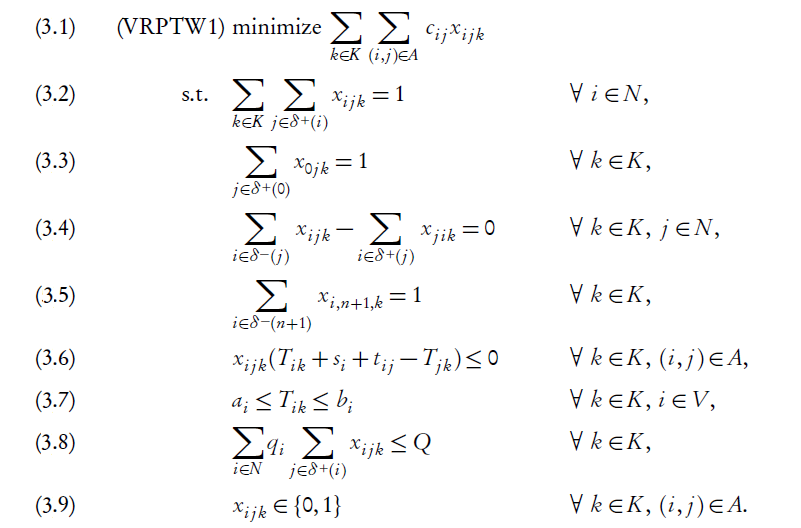
\includegraphics[scale=0.7]{figuras/math1.PNG}
\label{math1}
\end{figure}



função objetivo (3.1) visa minimizar o custo total. As restrições (3.2) garantem que cada cliente é atribuído a exatamente um percurso.Em seguida, as restrições (3.3) - (3.5) definem um caminho da \textit{source-to-sink} no G para cada k veículo.Além disso, as restrições (3.6) - (3.7) e a viabilidade do cronograma (3.8) garantia em relação à janelas de tempo e capacidade do veículo, respetivamente. Finalmente, os arcos de fluxo estão sujeitos a requisitos binários (3.9).

Modelo (3.1) - (3.9) é não linear devido as restrições de (3.6) que pode, no entanto, ser linearizada como: 

\begin{figure}[ht!]
\centering
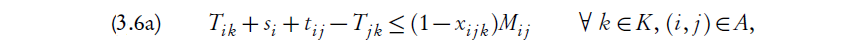
\includegraphics[scale=0.7]{figuras/math6.PNG}
\label{math6}
\end{figure}

Onde $ M_{ij}$ , (i, j ) $\in$ A, são grandes constantes que podem ser definidas para  $ max \{b_i + s_i +t_{ij} - a_j , 0 \}$



O relaxamento linear do modelo (3.1) - (3.5), (3.6a), (3.7) - (3.9) prevê, em geral, limites inferiores muito fracos . Este modelo tem, no entanto, uma estrutura de bloco-angular que pode ser explorada, onde cada bloco é composto das restrições (3.3) - (3.5), (3.6a), (3.7) - (3.9) para um veículo específico, k $\in$ K e define um Problema do Caminho Mais Curto Elementar com restrições de recursos (ESPPRC). Aplicando o princípio de decomposição de Dantzig-Wolfe \cite{gendreau01} para este modelo produz o seguinte modelo de particionamento definida uma vez que os veículos (idênticos) e suas variáveis correspondentes são agregados \cite{gendreau10}. Neste modelo,$\omega$ denota o conjunto de todas as rotas possíveis, $c_r$ o custo da rota r $\in$ $\omega$ and $a_{ir}$ o número de visitas ao cliente i $\in$ N em rota r $\in$ $\omega$ ($a_{ir}$ $\in$ {0,1}, quando r é uma rota fundamental. Com cada rota r $\in$ $\omega$ está associado um ano variável de caminho binária que assume valor 1 se rota r é selecionado na solução e 0 caso contrário. o modelo de partição do conjunto é

\begin{figure}[ht!]
\centering
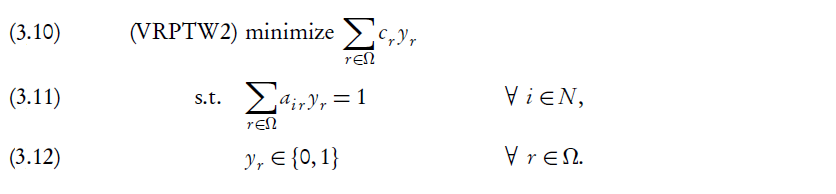
\includegraphics[scale=0.7]{figuras/math2.PNG}
\label{math2}
\end{figure}



função objetivo (3.10) procura minimizar o custo total. Definir restrições de particionamento (3.11) impõem que cada cliente ser visitada apenas uma vez por um veículo. Os requisitos binários nas variáveis caminho de fluxo são expressos por (3.12). Note-se que, como na literatura PRVJT, o modelo acima assume que o número de veículos disponível para atender os clientes é ilimitada, isto é, |k| é tão grande quanto necessário. Se este não foi o caso, a restrição de aplicar a seleção de, no máximo, uma rota disponível por veículo iria ser adicionado ao modelo.

\begin{figure}[ht!]
\centering
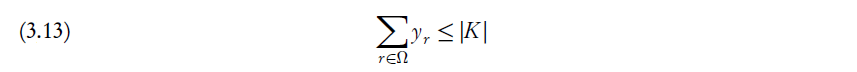
\includegraphics[scale=0.7]{figuras/math3.PNG}
\label{math3}
\end{figure}
 
 
O relaxamento linear do modelo (3.10) - (3.12) produz uma melhor limites mais baixos do que a do modelo (3.1) - (3.5), (3.6a), (3.7) - (3.9). Por outro lado, o modelo de partição do conjunto contém um grande número de variáveis, por rota viável.% No ponto 3.3.1, 

Vários outros modelos foram propostos para a PRVJT. Em particular, as formulações de dois índices foram usados em conjunto com algoritmos Branch-and-CUT . Apresenta-se uma tal formulação abaixo, que envolve um tipo de variáveis: para cada arco (i, j) $\in$ A, existe um binário variável $x_{ij}$ que é igual a 1 se o arco (i, j) é utilizada em solução e 0 se não for usado. Denote por P o conjunto de caminhos (não necessariamente a partir da origem) em G que não respeitam as restrições de janela de tempo e por A (p) o conjunto de arcos no caminho p$\in$ P. Deixe r(S) o número mínimo de veículos necessários para servir cada subconjunto de clientes S de acordo com suas demandas. Este número é, em geral, substituídos por $[q(S)/Q]$ em $q(S)=\sum\limits_{i \in S}q_i $. A formulação de duas índice corresponde à 

\begin{figure}[ht]
\centering
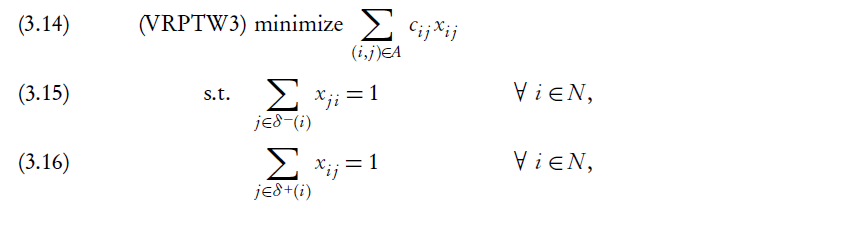
\includegraphics[scale=0.7]{figuras/math4.PNG}
\label{math4}
\end{figure}

\begin{figure}[ht]
\centering
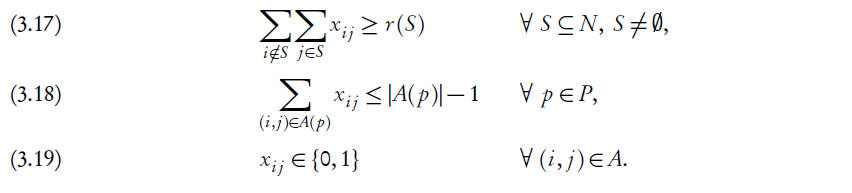
\includegraphics[scale=0.7]{figuras/math5.PNG}
\label{math5}
\end{figure}

função objetivo (3.14) minimiza o custo total para servir os clientes. Restrições (3.15) - (3.16) garantir que um veículo chega e sai de cada cliente, respectivamente. desigualdades de capacidade (3.17) garantir que a capacidade do veículo está satisfeito em todas as rotas selecionadas e também força o relaxamento linear através da imposição de um número mínimo de veículos para atender cada subconjunto de clientes S. Além disso, eles agem como restrições de eliminação sub deslocamento. desigualdades caminho inviável (3.18) proibir a seleção de caminhos que não respeitam as janelas de tempo. Finalmente, as variáveis de fluxo $x_{ij}$ estão sujeitos a requisitos de binários (3.19).

 A formulação de dois índice (3.14) - (3.19) contém um número exponencial de restrições (3.17) e (3.18). Para os casos de tamanhos práticos , eles precisam ser gerados dinamicamente como no algoritmo de plano de corte. desigualdades válidas adicionais também podem ser considerados para apertar o relaxamento linear deste modelo
 


\subsection{Conjunto de Problemas Testes de Solomon}

 O conjunto de problemas teste proposto por Solomon em 1987 \cite{solomon87}, baseado  em  dados  de  alguns  problemas  usados  por  Christofides  et  al.  (1979)  para  o  problema de roteamento padrão, trata-se de diferentes classes de instâncias, cada qual com características   geográficas   e   de   restrições   características.   Os   consumidores   estão   distribuídos em um plano XY de dimensões 100x100.  



As instâncias são divididas em 6 grupos denominados R1, R2, C1, C2, RC1 e RC2. Cada classe contém entre 8 e 12 instâncias. Os grupos R1 e R2, possuem uma disposição geográfica dos clientes de forma aleatória, já nos grupos C1 e C2, a disposição é na forma de  agrupamentos,  e  nos  grupos  RC1  e  RC2  são  tipos  mistos  (parte  em  agrupamentos  e  parte  aleatória).  Nas  classes  R1,  C1  e  RC1,  as  janelas  de  tempo  e  o  horizonte  total  são  curtos, diminuindo assim o número de consumidores por rota. Já as classes R2, C2 e RC2, possuem  um  longo  horizonte  total  fazendo  com  que  as  rotas  tenham  mais  consumidores  viáveis.   


Cada instância tem 100 consumidores, mas pode-se considerar apenas os primeiros 25 ou 50 consumidores dependendo do caso. 



No caso do uso das instâncias de Solomon, nos problemas de roteamento dinâmico, adaptações devem ocorrer para que não se tenha  conhecimento  de  todos  os  consumidores  no início do roteamento, o que tornaria o problema estático.  




%As  figuras  abaixo,  representam  os  três  tipos  de  classe  C  (Fig.2.4),  R  (Fig.2.5)  e    RC(Fig.2.6): 

\begin{figure}[ht!]
	\centering
	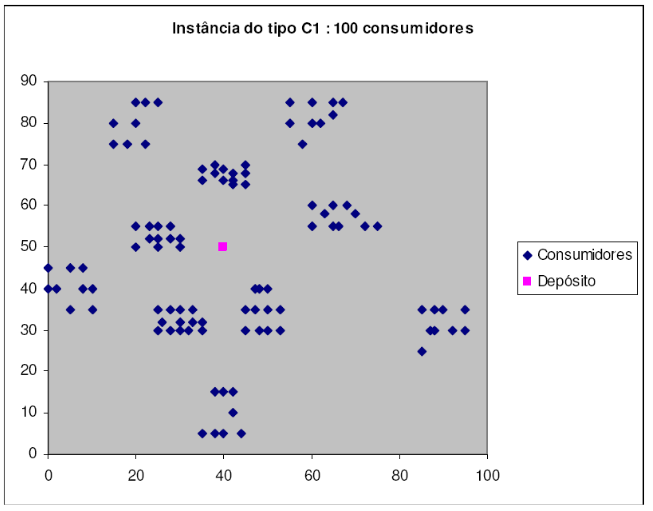
\includegraphics[scale=0.7]{figuras/solo1.PNG}
	\label{solo1}
	\caption{Problemas classe C}
\end{figure}

\begin{figure}[ht!]
	\centering
	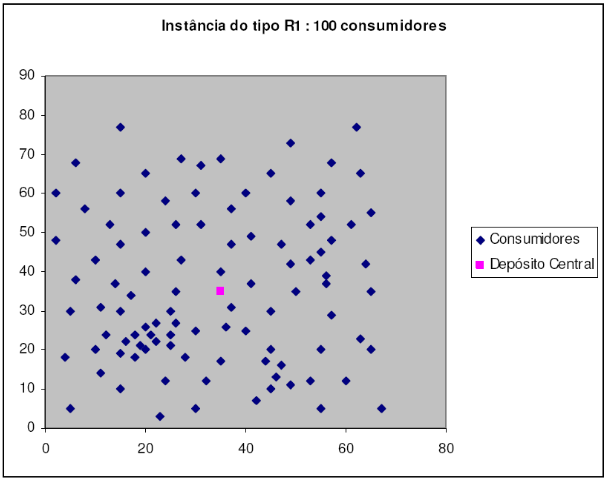
\includegraphics[scale=0.7]{figuras/solo2.PNG}
	\label{solo2}
	\caption{Problemas classe R}
\end{figure}

\begin{figure}[ht!]
	\centering
	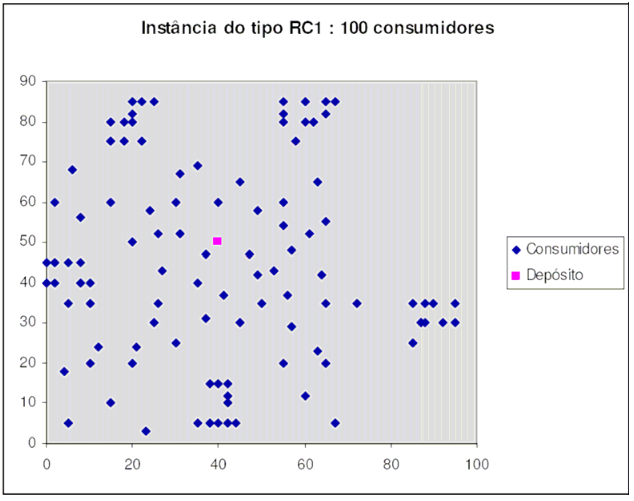
\includegraphics[scale=0.7]{figuras/solo3.PNG}
	\label{solo3}
	\caption{Problemas classe RC}
\end{figure}




\chapter{Conclusão}

Este documento e seu código-fonte são exemplos de referência de uso da classe
\textsf{abntex2} e do pacote \textsf{abntex2cite}. O documento 
exemplifica a elaboração de trabalho acadêmico (tese, dissertação e outros do
gênero) produzido conforme a ABNT NBR 14724:2011 \emph{Informação e documentação
- Trabalhos acadêmicos - Apresentação}.

A expressão ``Modelo Canônico'' é utilizada para indicar que \abnTeX\ não é
modelo específico de nenhuma universidade ou instituição, mas que implementa tão
somente os requisitos das normas da ABNT. Uma lista completa das normas
observadas pelo \abnTeX\ é apresentada em \citeonline{abntex2classe} \cite{abntex2classe}.

Sinta-se convidado a participar do projeto \abnTeX! Acesse o site do projeto em
\url{http://www.abntex.net.br/}. Também fique livre para conhecer,
estudar, alterar e redistribuir o trabalho do \abnTeX, desde que os arquivos
modificados tenham seus nomes alterados e que os créditos sejam dados aos
autores originais, nos termos da ``The \LaTeX\ Project Public
License''\footnote{\url{http://www.latex-project.org/lppl.txt}}.

Encorajamos que sejam realizadas customizações específicas deste exemplo para
universidades e outras instituições --- como capas, folha de aprovação, etc.
Porém, recomendamos que ao invés de se alterar diretamente os arquivos do
\abnTeX, distribua-se arquivos com as respectivas customizações.
Isso permite que futuras versões do \abnTeX~não se tornem automaticamente
incompatíveis com as customizações promovidas. Consulte
\citeonline{abntex2-wiki-como-customizar} par mais informações.

Este documento deve ser utilizado como complemento dos manuais do \abnTeX\ 
\cite{abntex2classe,abntex2cite,abntex2cite-alf} e da classe \textsf{memoir}
\cite{gendreau10}. 

Esperamos, sinceramente, que o \abnTeX\ aprimore a qualidade do trabalho que
você produzirá, de modo que o principal esforço seja concentrado no principal:
na contribuição científica.

Equipe \abnTeX 

Lauro César Araujo





% -----------------------------------------------------------------
% ELEMENTOS PÓS-TEXTUAIS
% -----------------------------------------------------------------
\postextual

% Você pode comentar os elementos que não deseja em seu trabalho;

% Referências bibliográficas
\bibliography{abntex2-modelo-references}	% Elemento Obrigatório
%% ----------------------------------------------------------
% Glossário
% ----------------------------------------------------------

Consulte o manual da classe abntex2 para orientações sobre o glossário.

\glossary
			% Elemento Opcional

% ----------------------------------------------------------
% Apêndices
% ----------------------------------------------------------

% ---
% Inicia os apêndices
% ---
\begin{apendicesenv}

% Imprime uma página indicando o início dos apêndices
\partapendices

% ----------------------------------------------------------
\chapter{Quisque libero justo}
% ----------------------------------------------------------

\lipsum[50]

% ----------------------------------------------------------
%\chapter{Nullam elementum urna vel imperdiet sodales elit ipsum pharetra ligula
%ac pretium ante justo a nulla curabitur tristique arcu eu metus}
%% ----------------------------------------------------------
%\lipsum[55-57]

\end{apendicesenv}
% ---				% Elemento Opcional

% ----------------------------------------------------------
% Anexos
% ----------------------------------------------------------
%
% ---
% Inicia os anexos
% ---
\begin{anexosenv}

% Imprime uma página indicando o início dos anexos
\partanexos
% ---
\chapter{Morbi ultrices rutrum lorem.}
% ---
\lipsum[30]

% ---
%\chapter{Cras non urna sed feugiat cum sociis natoque penatibus et magnis dis
%parturient montes nascetur ridiculus mus}
%% ---
%
%\lipsum[31]
%
%% ---
%\chapter{Fusce facilisis lacinia dui}
%% ---
%
%\lipsum[32]

\end{anexosenv}
				% Elemento Opcional
%
%%---------------------------------------------------------------------
%% INDICE REMISSIVO
%%---------------------------------------------------------------------
\phantompart
\printindex
%---------------------------------------------------------------------

		% Elemento Opcional

\end{document}

% -----------------------------------------------------------------
% Fim do Documento
% -----------------------------------------------------------------	